\documentclass{article}
\usepackage{amsthm,amsmath, amssymb, fullpage, hyperref, tikz, caption}

\begin{document}

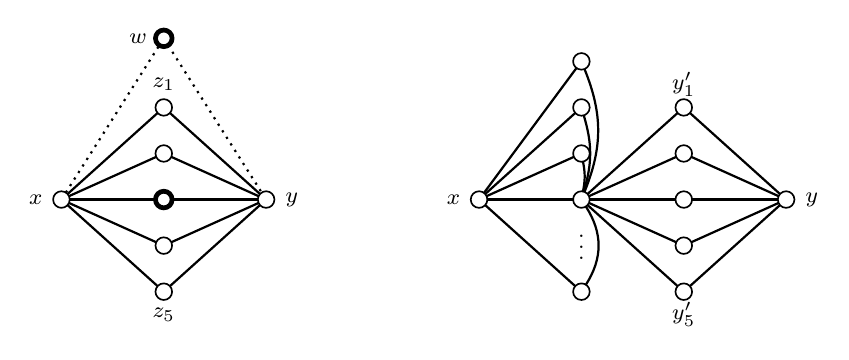
\begin{tikzpicture}[thick, scale=.65, yscale=.9]
\tikzstyle{uStyle}=[shape = circle, minimum size = 6pt, inner sep = 0pt,
outer sep = 0pt, draw, fill=white, semithick]
\tikzstyle{sStyle}=[shape = rectangle, minimum size = 4.5pt, inner sep = 0pt,
outer sep = 0pt, draw, fill=white, semithick]
\tikzstyle{lStyle}=[shape = circle, minimum size = 4.5pt, inner sep = 0pt,
outer sep = 0pt, draw=none, fill=none]
\tikzset{every node/.style=uStyle}
\def\rad{2.5cm}
\def\off{.5cm}

\foreach \i in {1,...,5}
\draw (0,3-\i) node (z\i) {};

\draw (-2,0) node (x) {} (2,0) node (y) {};

\foreach \i in {1,...,5}
\draw (x) -- (z\i) -- (y);

\draw (x) ++ (-\off,0) node[lStyle] {\footnotesize{$x$}};
\draw (y) ++ (\off,0) node[lStyle] {\footnotesize{$y$}};
\draw (z1) ++ (0,\off) node[lStyle] {\footnotesize{$z_1$}};
\draw (z5) ++ (0,-\off) node[lStyle] {\footnotesize{$z_5$}};
\draw (0,3.5) node[line width=.6mm] (w) {} ++ (-\off,0) node[lStyle] {\footnotesize{$w$}};
\draw (z3) node[line width=.6mm] {};
\draw[dotted] (x) -- (w) -- (y);

\begin{scope}[xshift=4in]

\foreach \i in {1,...,5}
\draw (0,3-\i) node (y\i) {};

\draw  (-4,0) node (x) {} -- (-2,0) node (x4) {} (2,0) node (y) {};

\foreach \i in {1,...,5}
\draw (x4) -- (y\i) -- (y);

\foreach \i in {1,2,3,6}
\draw (-2,4-\i) node (x\i) {} -- (x);

\draw (x4) edge[bend right=20] (x1);
\draw (x4) edge[bend right=15] (x2);
\draw (x4) edge[bend right=10] (x3);
\draw (-2,-.85) node[lStyle] {\footnotesize{$\vdots$}};
\draw (x4) edge[bend left] (x6);

\draw (x) ++ (-\off,0) node[lStyle] {\footnotesize{$x$}};
\draw (y) ++ (\off,0) node[lStyle] {\footnotesize{$y$}};
\draw (y1) ++ (0,\off) node[lStyle] {\footnotesize{$y'_1$}};
\draw (y5) ++ (0,-\off) node[lStyle] {\footnotesize{$y'_5$}};
\end{scope}
\end{tikzpicture}

\end{document}